\chapter{Cài đặt, vận hành và bảo trì}
\label{chap:install}
\section{Kiến trúc triển khai}
Ứng dụng gồm SPA React/Vite trong \path{store-admin/client}, API Express trong \path{store-admin/server}, PostgreSQL và Kafka. Khi chạy server chế độ phục vụ client, server trả static build từ \path{client/dist}. Môi trường local có Docker Compose cho PostgreSQL và Kafka; Kafka UI chỉ phục vụ quan sát. PostgreSQL/Kafka managed có cấu hình riêng, cần cung cấp biến môi trường và chứng thư qua cơ chế bảo mật của nền tảng.

\IfFileExists{diagrams/05-trien-khai-su-kien.pdf}{\begin{figure}[htbp]\centering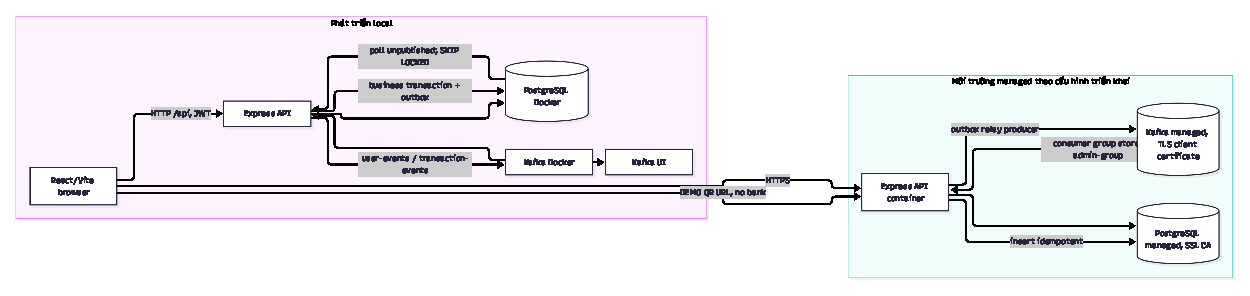
\includegraphics[width=0.96\textwidth]{diagrams/05-trien-khai-su-kien.pdf}\caption{Triển khai và luồng sự kiện outbox/Kafka}\label{fig:deployment}\end{figure}}{\begin{figure}[htbp]\centering\fbox{\parbox[c][2cm][c]{0.82\textwidth}{\centering Cần kết xuất Mermaid từ \texttt{diagrams/05-trien-khai-su-kien.mmd}}}\caption{Triển khai và luồng sự kiện outbox/Kafka}\label{fig:deployment}\end{figure}}

\section{Cài đặt môi trường local}
Các lệnh dưới đây dựa trên scripts đã có trong \texttt{\detokenize{store-admin/package.json}}. Chuẩn bị Node.js/npm, Docker Desktop, PostgreSQL client tools nếu cần backup/restore và file môi trường local do người vận hành tự tạo từ danh sách biến trong \texttt{\detokenize{server/.env.example}}. Không đưa file môi trường thật vào source archive.
\begin{enumerate}
\item Tại thư mục \texttt{\detokenize{store-admin}}, cài phụ thuộc bằng \texttt{\detokenize{npm install}}.
\item Khởi chạy dịch vụ local PostgreSQL/Kafka và frontend/backend bằng \texttt{\detokenize{npm run dev:local}}; hoặc khởi động dịch vụ qua Compose rồi chạy \texttt{\detokenize{npm run dev}}.
\item Chạy migration bằng \texttt{\detokenize{npm run db:migrate --workspace server}}.
\item Nếu cần dữ liệu mẫu, đặt \texttt{\detokenize{SEED_DEMO_PASSWORD}} trong môi trường shell (8--72 byte UTF-8, không ghi vào file/log), rồi chạy \texttt{\detokenize{npm run seed}}. Script chỉ in xác nhận biến đã được dùng, không in giá trị mật khẩu. Seed có thể truy cập nguồn catalog bên ngoài; chỉ chạy trong local/test.
\item Để có thêm event, lịch sử điểm, gán khuyến mãi và hội thoại mẫu, chạy \texttt{\detokenize{node scripts/seed-report-demo.mjs}} sau seed chính; script yêu cầu các biến \texttt{\detokenize{SEED_DB_*}} trỏ về loopback.
\item Tạo production client build bằng \texttt{\detokenize{npm run build}}; chạy server bằng \texttt{\detokenize{npm start}} theo script hiện có.
\end{enumerate}

\section{Cấu hình biến môi trường}
Bảng liệt kê tên biến từ \texttt{\detokenize{server/.env.example}} và cách đọc trong mã nguồn; không chứa giá trị. Dùng secret manager của nền tảng cho bí mật. \texttt{\detokenize{TRUST_PROXY_HOPS}} mặc định local nên giữ 0; chỉ cấu hình số hop phù hợp khi triển khai sau proxy tin cậy. Cấu hình demo payment và URL công khai chỉ bật trong môi trường trình diễn, tuyệt đối không coi QR demo là giao dịch ngân hàng.
\small
\begin{longtable}{|p{0.45\textwidth}|p{0.42\textwidth}|}\hline
\textbf{Tên biến}&\textbf{Mục đích}\\
\hline\endhead
\texttt{\detokenize{PORT}}, \texttt{\detokenize{LOCAL_HOST}}&Cổng và địa chỉ bind của HTTP server.\\
\hline
\texttt{\detokenize{JWT_SECRET}}&Chữ ký token đăng nhập; bí mật, tự cấp riêng cho môi trường.\\
\hline
\texttt{\detokenize{TRUST_PROXY_HOPS}}&Số proxy hop tin cậy khi xác định IP; chỉ tăng khi đã xác minh topology.\\
\hline
\texttt{\detokenize{AUTH_RATE_LIMIT_WINDOW_MS}}, \texttt{\detokenize{AUTH_LOGIN_RATE_LIMIT_MAX}}, \texttt{\detokenize{AUTH_REGISTER_RATE_LIMIT_MAX}}&Cửa sổ và ngưỡng giới hạn login/đăng ký.\\
\hline
\texttt{\detokenize{POSTGRES_HOST}}, \texttt{\detokenize{POSTGRES_PORT}}, \texttt{\detokenize{POSTGRES_DB}}, \texttt{\detokenize{POSTGRES_USER}}, \texttt{\detokenize{POSTGRES_PASSWORD}}&Kết nối PostgreSQL; mật khẩu là bí mật.\\
\hline
\texttt{\detokenize{POSTGRES_SSL}}, \texttt{\detokenize{POSTGRES_CA_PATH}}&TLS và CA cho PostgreSQL managed, nếu cấu hình yêu cầu.\\
\hline
\texttt{\detokenize{PG_DUMP_PATH}}, \texttt{\detokenize{PG_RESTORE_PATH}}&Đường dẫn PostgreSQL client tools.\\
\hline
\texttt{\detokenize{KAFKA_BROKER}}, \texttt{\detokenize{KAFKA_BROKERS}}, \texttt{\detokenize{KAFKA_UI_PORT}}&Bootstrap broker(s) và cổng UI local.\\
\hline
\texttt{\detokenize{KAFKA_SSL_CA}}, \texttt{\detokenize{KAFKA_SSL_CA_PATH}}, \texttt{\detokenize{KAFKA_SSL_CERT}}, \texttt{\detokenize{KAFKA_SSL_CERT_PATH}}, \texttt{\detokenize{KAFKA_SSL_KEY}}, \texttt{\detokenize{KAFKA_SSL_KEY_PATH}}&TLS/mTLS Kafka; đường dẫn chứng thư/khóa không phải dữ liệu đưa vào báo cáo.\\
\hline
\texttt{\detokenize{DEMO_PAYMENT}}, \texttt{\detokenize{PUBLIC_BASE_URL}}&Bật luồng thanh toán demo và URL mà điện thoại truy cập được. Không kết nối ngân hàng.\\
\hline
\texttt{\detokenize{ENABLE_DATABASE_BROWSER}}, \texttt{\detokenize{ENABLE_DATABASE_RESTORE}}&Bật các công cụ quản trị dữ liệu; chỉ bật có kiểm soát và trong môi trường phù hợp.\\
\hline
\texttt{\detokenize{PYTHON_EXECUTABLE}}&Python executable được script catalog dùng khi cần.\\
\hline
\texttt{\detokenize{EVENT_RATE_LIMIT_WINDOW_MS}}, \texttt{\detokenize{EVENT_RATE_LIMIT_MAX}}&Giới hạn route thu nhận event.\\
\hline
\texttt{\detokenize{OUTBOX_MAX_BACKLOG}}, \texttt{\detokenize{KAFKA_DB_CONFIRM_TIMEOUT_MS}}&Ngưỡng backlog và thời gian chờ xác nhận consumer.\\
\hline
\texttt{\detokenize{DEBUG_CHAT_SSE}}, \texttt{\detokenize{CHAT_UPLOAD_DIR}}&Log chẩn đoán SSE và thư mục lưu file chat.\\
\hline
\end{longtable}
\normalsize

\section{Chạy migration và khởi tạo dữ liệu}
Schema ban đầu nằm ở \texttt{\detokenize{server/sql/schema.sql}}; migrations 001--015 được thực thi theo runner. \texttt{\detokenize{database/schema.sql}} là dump schema-only và \texttt{\detokenize{database/demo-data.sql}} là dump data-only sinh từ database local đã seed ngày 03/11/2026. Hai file đã được nạp lần lượt vào database rỗng; row count khớp trên 40/40 bảng. Dump data chứa hash bcrypt của mật khẩu các tài khoản demo; không chứa mật khẩu dạng rõ. Mật khẩu rõ chỉ được cung cấp khi chạy seed qua biến môi trường.

Sau lần chạy riêng \texttt{\detokenize{npm run seed}} trước khi bổ sung seed báo cáo, các bảng rỗng là:
\begin{itemize}
\item \texttt{conversation}, \texttt{chat\_message}, \texttt{chat\_message\_attachment}, \texttt{demo\_payment\_tokens}, \texttt{feedback\_attachment};
\item \texttt{loyalty\_point\_transaction}, \texttt{outbox\_events}, \texttt{transactions}, \texttt{user\_events}, \texttt{user\_promotion}.
\end{itemize}
Sau khi chạy thêm seed báo cáo, chỉ còn \texttt{demo\_payment\_tokens} (token dùng một lần, chỉ tồn tại trong checkout demo đang hoạt động) và hai bảng đính kèm (chỉ phát sinh khi người dùng tải file thật vào chat/phản hồi) rỗng. Schema hiện không có bảng \texttt{task}, vì vậy chưa thể tạo bản ghi công việc nếu không bổ sung nghiệp vụ/schema.

\section{Backup, phục hồi và an toàn dữ liệu}
\label{sec:backup-restore}
Ngày 03/11/2026, nhóm thực hiện drill trên PostgreSQL 16 Alpine trong container Docker tạm chỉ bind vào loopback; không kết nối dịch vụ managed. Lệnh dump custom format: \texttt{\detokenize{docker exec hf-report-pg-20261103 pg_dump -Fc -U report_user -d report_demo -f /tmp/report-demo.dump}}; thời gian đo tại máy chạy Docker là 0,276 giây, kích thước dump 161,9 KiB. Tạo database đích rỗng bằng \texttt{\detokenize{docker exec hf-report-pg-20261103 createdb -U report_user report_restore}} mất 0,186 giây. Lệnh phục hồi \texttt{\detokenize{docker exec hf-report-pg-20261103 pg_restore -U report_user -d report_restore --no-owner --no-privileges /tmp/report-demo.dump}} mất 3,860 giây. Sau restore, truy vấn COUNT trên từng bảng public cho kết quả bằng nhau ở 40/40 bảng (0 sai khác). Đây là một lần đo trên máy local, không phải cam kết RTO cho production.

Đối chiếu row count từng bảng (nguồn = database đã seed; đích = database restore):
\scriptsize
\begin{longtable}{|p{0.55\textwidth}|r|r|}\hline
\textbf{Bảng}&\textbf{Nguồn}&\textbf{Restore}\\\hline\endhead
account&10&10\\\hline
brand&1&1\\\hline
category&9&9\\\hline
chat\_message&6&6\\\hline
chat\_message\_attachment&0&0\\\hline
color&8&8\\\hline
conversation&3&3\\\hline
customer&26&26\\\hline
customer\_interest&23&23\\\hline
demo\_payment\_tokens&0&0\\\hline
employee&6&6\\\hline
feedback&12&12\\\hline
feedback\_attachment&0&0\\\hline
import\_detail&180&180\\\hline
import\_receipt&1&1\\\hline
interest&8&8\\\hline
loyalty\_point\_transaction&20&20\\\hline
order&41&41\\\hline
order\_detail&82&82\\\hline
outbox\_events&4&4\\\hline
payment&41&41\\\hline
permission&12&12\\\hline
product&180&180\\\hline
product\_image&180&180\\\hline
product\_variant&180&180\\\hline
promotion&3&3\\\hline
role&6&6\\\hline
role\_permission&27&27\\\hline
size&13&13\\\hline
store\_admin\_schema\_migrations&16&16\\\hline
supplier&4&4\\\hline
survey&1&1\\\hline
survey\_answer&15&15\\\hline
survey\_invitation&8&8\\\hline
survey\_option&3&3\\\hline
survey\_question&3&3\\\hline
survey\_response&5&5\\\hline
transactions&4&4\\\hline
user\_events&3&3\\\hline
user\_promotion&8&8\\\hline
\end{longtable}
\normalsize

\section{Kế hoạch chuyển đổi và triển khai môi trường demo}
Môi trường demo sử dụng PostgreSQL managed với SSL và xác minh CA, cùng Kafka managed trên Aiven với xác thực client certificate qua cổng SSL. Hai topic \texttt{\detokenize{user-events}} và \texttt{\detokenize{transaction-events}} được tạo trước; cấu hình auto-create topic tắt. Không ghi hostname, chuỗi kết nối, mật khẩu, token hay nội dung chứng thư trong tài liệu. Người vận hành lấy giá trị từ các biến môi trường tương ứng và kho bí mật của nền tảng.
\begin{enumerate}
\item Đóng băng thay đổi dữ liệu ở nguồn local, xác nhận phiên bản schema/migration và tạo bản dump PostgreSQL dạng custom bằng \texttt{\detokenize{pg_dump -Fc}}.
\item Kiểm tra checksum và quyền truy cập bản backup; chuẩn bị PostgreSQL đích, CA tin cậy, tài khoản giới hạn quyền, Kafka SSL client credentials và tạo trước hai topic với cấu hình retention/partition đã thống nhất.
\item Khôi phục dữ liệu lên PostgreSQL managed bằng \texttt{\detokenize{pg_restore --no-owner --no-privileges}}; không thay đổi bản nguồn. Cấu hình ứng dụng qua secret manager/biến môi trường, xác minh CA và xác thực Kafka trước khi chuyển lưu lượng.
\item So sánh số hàng của từng bảng nguồn/đích, kiểm tra constraints và migration version; xác nhận backlog outbox được relay, consumer xử lý được transaction event, rồi chạy smoke test đăng nhập, đọc dữ liệu, tạo đơn thử nghiệm và luồng QR demo.
\item Chuyển lưu lượng sau khi đối chiếu hoàn tất. Theo dõi lỗi API, kết nối SSL, Kafka consumer lag và outbox backlog trong thời gian đầu.
\end{enumerate}
Nếu kiểm tra sau chuyển đổi thất bại, người phụ trách triển khai tạm dừng thao tác ghi, giữ nguyên nguồn local và bản backup, chuyển cấu hình ứng dụng về nguồn trước đó, rồi đối chiếu các thay đổi phát sinh sau thời điểm dump trước khi mở lại ghi. Không phục hồi đè lên môi trường managed đang có dữ liệu mới mà chưa có quyết định và bản sao lưu phù hợp.

Phân công tối thiểu: quản trị CSDL chịu trách nhiệm backup/restore, CA, quyền truy cập và đối chiếu số hàng; người vận hành triển khai chịu trách nhiệm biến môi trường, chứng thư Kafka, topic và chuyển lưu lượng; người điều phối nhóm ghi nhận thời điểm chuyển đổi và phê duyệt kết quả. Tên người và biên bản thực tế cần được nhóm bổ sung.

\section{Vận hành Kafka và thanh toán demo}
Outbox writer ghi sự kiện cùng giao dịch nghiệp vụ. Relay lấy bản ghi chưa gửi bằng khóa hàng \texttt{\detokenize{SKIP LOCKED}}, gửi theo topic, rồi đánh dấu \texttt{\detokenize{published_at}}; nếu gửi thành công nhưng chưa kịp đánh dấu, có thể phát lại. Consumer dùng \texttt{\detokenize{event_id}} để chống ghi lặp. Các topic nghiệp vụ hiện có là \texttt{\detokenize{user-events}} và \texttt{\detokenize{transaction-events}}; trong demo chúng phải được tạo trước, auto-create tắt.

Thanh toán DEMO phát token ngẫu nhiên dùng một lần, hết hạn sau 15 phút, lưu dạng băm; trang công khai ghi rõ đây không phải giao dịch thật. \texttt{\detokenize{PUBLIC_BASE_URL}} cần trỏ tới địa chỉ LAN/tunnel truy cập được từ điện thoại trong buổi demo. Không bật trên môi trường giao dịch thật; cơ chế này không đối soát với ngân hàng.

\subsection{Ảnh minh chứng triển khai}
Ảnh minh chứng được tự động nhúng nếu đặt trong \texttt{\detokenize{docs/report/images}} theo đúng tên dưới đây.
\ReportScreenshot{5.1}{Sơ đồ môi trường triển khai dùng cho buổi demo}{fig:deployment-screenshot}
\ReportScreenshot{5.2}{Checkout QR DEMO và trang xác nhận không phải giao dịch thật}{fig:demo-payment-screenshot}

\section{Giới hạn free tier}
Không ấn định một giới hạn throughput hoặc topic chung cho gói free: hạn mức thay đổi theo nhà cung cấp, khu vực và loại dịch vụ. Nhóm cần ghi lại các giới hạn hiển thị trong console đúng ngày demo: [CẦN BỔ SUNG: số liệu và ngày]. Hình~\ref{fig:quota-console} là vị trí chờ ảnh console đã che thông tin định danh/credential. Nếu thấy lỗi giới hạn số topic, kiểm tra quota/ACL và số topic thực tế, sau đó gộp hoặc xóa topic chỉ theo quyết định quản trị cluster. Không xóa topic có dữ liệu cần giữ.
\ReportScreenshot{5.3}{Giới hạn gói hiển thị trong console tại ngày demo (Chờ ảnh)}{fig:quota-console}

\section{Ma trận chức năng theo vai trò}
Ma trận giao diện lấy từ route visibility ở \texttt{\detokenize{client/src/App.jsx}}; API còn kiểm tra vai trò ở middleware/route.
\small
\begin{longtable}{|p{0.22\textwidth}|p{0.65\textwidth}|}\hline
\textbf{Vai trò}&\textbf{Phạm vi chính theo ứng dụng}\\
\hline\endhead
ADMIN&Quản trị tài khoản và phân quyền; truy cập các module quản trị, báo cáo, cài đặt theo quyền được triển khai.\\
\hline
QL\_NHAN\_SU&Chức năng nhân sự/tài khoản được phân quyền trong dashboard; không có bằng chứng module chấm công, lương, nghỉ phép đầy đủ.\\
\hline
QL\_KHO&Sản phẩm, kho, nhà cung cấp và các chức năng vận hành kho được router/UI cho phép.\\
\hline
QL\_BAN\_HANG&Đơn hàng/bán hàng theo router/UI; một số báo cáo và xử lý đơn phụ thuộc quyền API.\\
\hline
QL\_KHACH\_HANG&Khách hàng, phản hồi, khảo sát và chat CSKH.\\
\hline
KHACH\_HANG&Portal: hồ sơ, đơn hàng, đánh giá, khảo sát và chat của chính khách hàng.\\
\hline
\end{longtable}
\normalsize

\section{Hướng dẫn sử dụng}
Các bước dưới đây bám theo màn hình và route hiện có. Menu có thể khác theo role; API tiếp tục kiểm tra quyền ở máy chủ. Tài khoản demo phải được cấp trước, đăng nhập bằng tên đăng nhập/email và mật khẩu do người quản trị cung cấp.

\subsection*{Đăng nhập chung}
\begin{enumerate}
\item Mở địa chỉ ứng dụng, nhập tên đăng nhập hoặc email cùng mật khẩu, chọn \textbf{Đăng nhập}.
\item Nếu tài khoản bị khóa hoặc thông tin không hợp lệ, liên hệ quản trị viên; không thử lặp liên tục vì đăng nhập có giới hạn số lần.
\item Sau khi vào hệ thống, sử dụng menu đúng phạm vi vai trò; đăng xuất từ menu hồ sơ khi kết thúc.
\end{enumerate}

\subsection*{ADMIN}
\begin{enumerate}
\item Mở \textbf{Tài khoản}, tìm tài khoản theo tên/email, tạo tài khoản với vai trò phù hợp hoặc dùng hộp xác nhận để đổi vai trò, khóa/mở khóa hay xóa khi đủ điều kiện.
\item Mở \textbf{Sản phẩm} hoặc \textbf{Tồn kho} để tra cứu sản phẩm/nhà cung cấp, xem thông tin và thực hiện thao tác quản trị được cấp.
\item Mở \textbf{Đơn hàng} để tra cứu đơn, xem chi tiết và xác nhận thanh toán theo nghiệp vụ; chỉ dùng QR DEMO nếu môi trường trình diễn đã bật.
\item Mở các mục \textbf{Khách hàng}, \textbf{Phản hồi}, \textbf{Khảo sát}, \textbf{Trò chuyện CSKH}, \textbf{Báo cáo} hoặc \textbf{Nhật ký} để theo dõi và xử lý dữ liệu tương ứng.
\end{enumerate}

\subsection*{QL\_KHO}
\begin{enumerate}
\item Đăng nhập và mở \textbf{Sản phẩm}; nhập từ khóa hoặc dùng bộ lọc đang hiển thị để tìm sản phẩm.
\item Mở \textbf{Tồn kho} để tra cứu nhà cung cấp/phiếu nhập và xem số lượng tồn; chỉ xác nhận nhập khi có chứng từ nghiệp vụ.
\item Dùng \textbf{Báo cáo} nếu mục này xuất hiện trong menu được cấp quyền; chức năng ngoài phạm vi menu cần quản trị viên hỗ trợ.
\end{enumerate}

\subsection*{QL\_BAN\_HANG}
\begin{enumerate}
\item Mở \textbf{Đơn hàng}, tìm đơn và xem trạng thái/chi tiết trước khi cập nhật.
\item Chọn phương thức thanh toán theo màn hình checkout. Với chuyển khoản demo, quét QR từ thiết bị khác và chờ trạng thái đơn cập nhật; mã này không đại diện giao dịch ngân hàng thật.
\item Mở \textbf{Khuyến mãi} để tra cứu hoặc quản lý khuyến mãi theo quyền; dùng \textbf{Báo cáo} để xem số liệu được cấp.
\end{enumerate}

\subsection*{QL\_KHACH\_HANG}
\begin{enumerate}
\item Mở \textbf{Khách hàng}, tìm hồ sơ, xem lịch sử và cập nhật thông tin theo quyền.
\item Mở \textbf{Phản hồi} để đọc, trả lời hoặc đổi trạng thái phản hồi; mở \textbf{Khảo sát} để tạo khảo sát, xem người nhận và kết quả.
\item Mở \textbf{Trò chuyện CSKH}, chọn hội thoại, gửi nội dung hoặc tệp được hỗ trợ, rồi cập nhật trạng thái xử lý.
\item Dùng báo cáo CRM, bao gồm thống kê tuổi ở `/api/customers/stats/overview` (trường `byAge`) hoặc `/api/reports/customer-ages`, nếu quyền API cho phép.
\end{enumerate}

\subsection*{QL\_NHAN\_SU}
\begin{enumerate}
\item Mở mục \textbf{Nhân viên} để tra cứu và quản lý hồ sơ nhân viên theo quyền được cấp.
\item Xem \textbf{Báo cáo} nếu có trong menu. Chức năng chấm công, tính lương và nghỉ phép chưa được xác nhận trong ứng dụng: [CẦN BỔ SUNG nếu thuộc yêu cầu đồ án].
\end{enumerate}

\subsection*{KHACH\_HANG}
\begin{enumerate}
\item Đăng nhập portal khách hàng; xem/cập nhật hồ sơ cá nhân và catalog sản phẩm.
\item Tạo đơn hàng, chọn phương thức thanh toán được cung cấp và theo dõi trạng thái đơn. QR DEMO chỉ mô phỏng: quét mã sẽ mở trang xác nhận demo, không chuyển tiền thật.
\item Gửi đánh giá/phản hồi, trả lời khảo sát được mời và nhắn CSKH trong hội thoại của chính mình.
\end{enumerate}

\section{Troubleshooting}
\begin{itemize}
\item Trang trống: kiểm tra console trình duyệt và terminal Vite; xác nhận build frontend và URL proxy \texttt{\detokenize{/api}}.
\item API không kết nối DB: xác nhận PostgreSQL chạy, host/port local khớp và migrations đã chạy; không chia sẻ thông tin kết nối khi gửi log.
\item Kafka không kết nối: kiểm tra broker reachable, ACL/topic và tên biến TLS; không gửi certificate/key trong issue hay ảnh chụp.
\item Điện thoại không mở QR demo: \texttt{\detokenize{PUBLIC_BASE_URL}} phải là IP LAN/tunnel có thể truy cập; host bind server cần reachable; không dùng \texttt{\detokenize{localhost}} của máy tính trong QR.
\item Backup/restore bị từ chối: script chỉ cho phép host local; không dùng script này để tác động database managed từ xa.
\end{itemize}
